\documentclass[12pt]{article}
\usepackage[margin=0.75in]{geometry} 
\usepackage{amsmath,amsthm,amssymb}
\usepackage{longtable}
\usepackage{mathtools}
\usepackage{standalone}
\usepackage{listings}
\usepackage{array}
\usepackage{float}
\usepackage{verbatim}
\usepackage{caption}
\usepackage{color} %red, green, blue, yellow, cyan, magenta, black, white
\usepackage{multicol}
\definecolor{mygreen}{RGB}{28,172,0} % color values Red, Green, Blue
\definecolor{mylilas}{RGB}{170,55,241}

\graphicspath{{../../Development/sensitivityTest/}}

% Set parameters for formatting imported Matlab
\lstset{language=Matlab,%
	basicstyle=\small
	%basicstyle=\color{red},
	breaklines=true,%
	morekeywords={matlab2tikz},
	keywordstyle=\color{blue},%
	morekeywords=[2]{1}, keywordstyle=[2]{\color{black}},
	identifierstyle=\color{black},%
	stringstyle=\color{mylilas},
	commentstyle=\color{mygreen},%
	showstringspaces=false,%without this there will be a symbol in the places where there is a space
	numbers=left,%
	numberstyle={\tiny \color{black}},% size of the numbers
	numbersep=9pt, % this defines how far the numbers are from the text
	emph=[1]{for,end,break},emphstyle=[1]\color{red}, %some words to emphasise
	%emph=[2]{word1,word2}, emphstyle=[2]{style},    
}

\title{Image Processing Sensitivity Analysis}
\author{Jack Cole}
\date{}

\begin{document}
	
\maketitle

\begin{multicols}{2}
	
\section{Introduction}

What questions are we trying to answer

The purpose of this analysis was to determine the sensitivity of the image processing software. Specifically, the Find6DOF block was tested in Simulink. This system is given inputs of the pixel locations of each white dot on the body of the BAT. The outputs of the system are the corresponding roll, pitch, and yaw Euler angles, as well as the center of mass position of the BAT. For the purpose of this analysis, solely the Euler angles were processed. In order to perform an accurate study, each pixel was modified separately and the corresponding change in Euler angle was observed.

\section{Methods}

How did we try to answer them

In the real system, each camera (side, bottom, and slant) captured four pixels location corresponding to the row and column of each pair of dots. The side and slant camera recorded only one pair of dots, while the bottom camera recorded two pairs of dots, denoted the A and B sets. The A set was lined up the x direction in the ground frame while the B set was lined up with the y direction in the ground frame.

In order to observe specific changes with regard to each dot location, each pixels was modified separately and the resulting Euler angles were plotted accordingly. More specifically, the row and column of each dot location were individually modified and plotted in reference to the change in Euler angle. To that end, sixteen separate graphs were plotted corresponding to changes with respect to each individual dot. Each plot describes the change in Euler angle versus the change in pixels. Each dot position was varied by $\pm 5$ pixels.

\section{Results}

Present the results. For example figure \ref{fig:botALeftCol} shows some stuff.

These graphs described how variations in dot location affected the Euler angles calculated by the Find6DOF block in Simulink. The results displayed show that some Euler angles are very sensitive to changes in pixel location 

% Side Camera Pixels

\begin{figure}[H]
	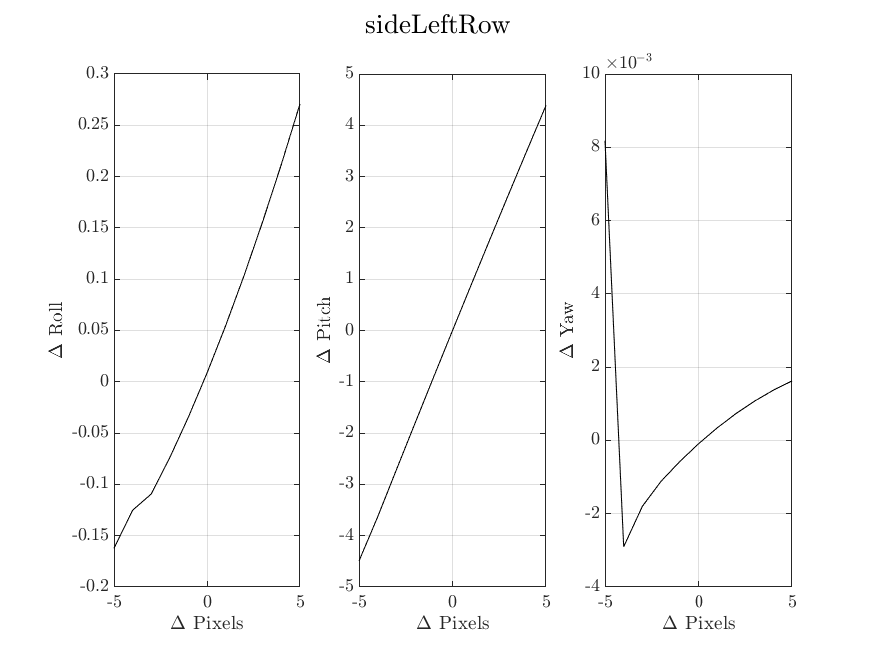
\includegraphics[width=0.9\columnwidth]{sideLeftRow.png}
	\caption{Side Camera Left Dot, Row\label{fig:sideLeftRow}}
\end{figure}

\begin{figure}[H]
	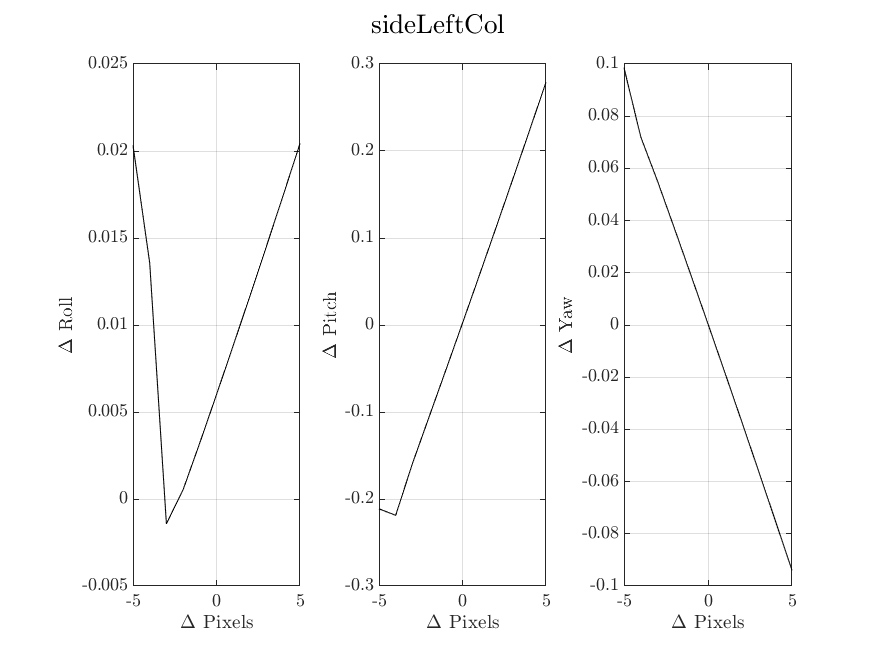
\includegraphics[width=0.9\columnwidth]{sideLeftCol.png}
	\caption{Side Camera Left Dot, Column\label{fig:sideLeftCol}}
\end{figure}

\begin{figure}[H]
	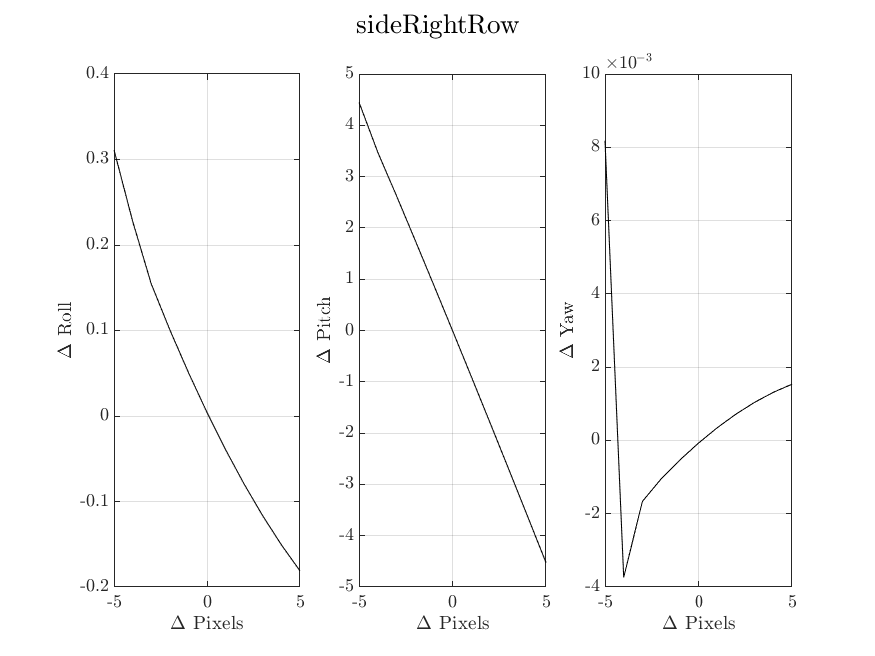
\includegraphics[width=0.9\columnwidth]{sideRightRow.png}
	\caption{Side Camera Right Dot, Row\label{fig:sideRightRow}}
\end{figure}

\begin{figure}[H]
	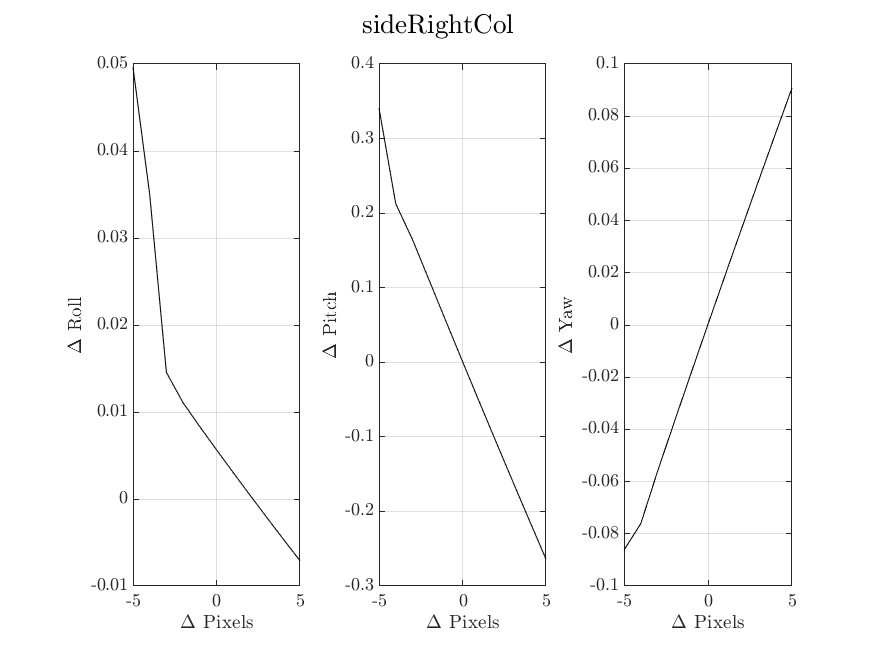
\includegraphics[width=0.9\columnwidth]{sideRightCol.png}
	\caption{Side Camera Right Dot, Column\label{fig:sideRightCol}}
\end{figure}

% Bottom A Camera Pixels

\begin{figure}[H]
	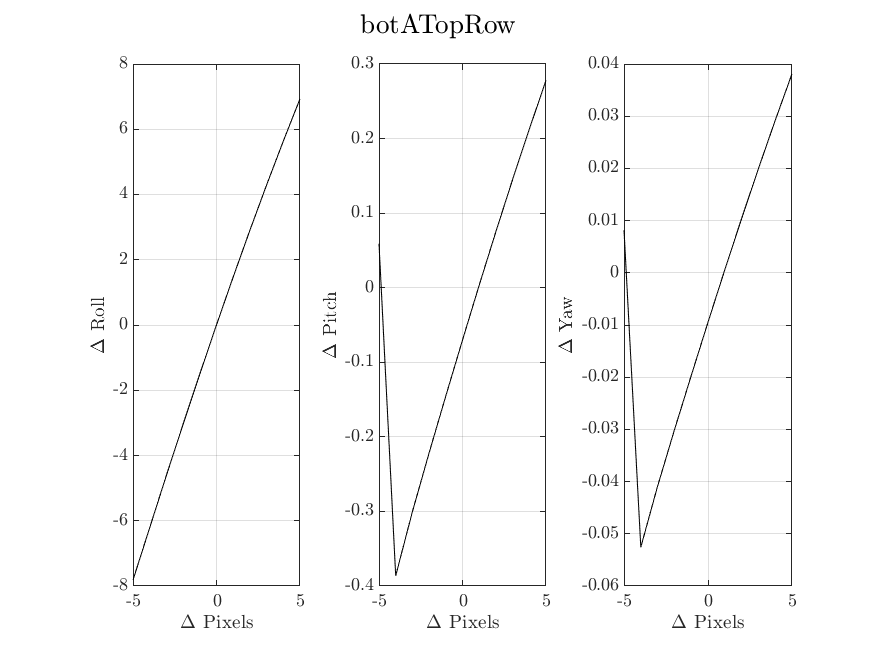
\includegraphics[width=0.9\columnwidth]{botATopRow.png}
	\caption{Bottom A Camera Top Dot, Row\label{fig:botATopRow}}
\end{figure}

\begin{figure}[H]
	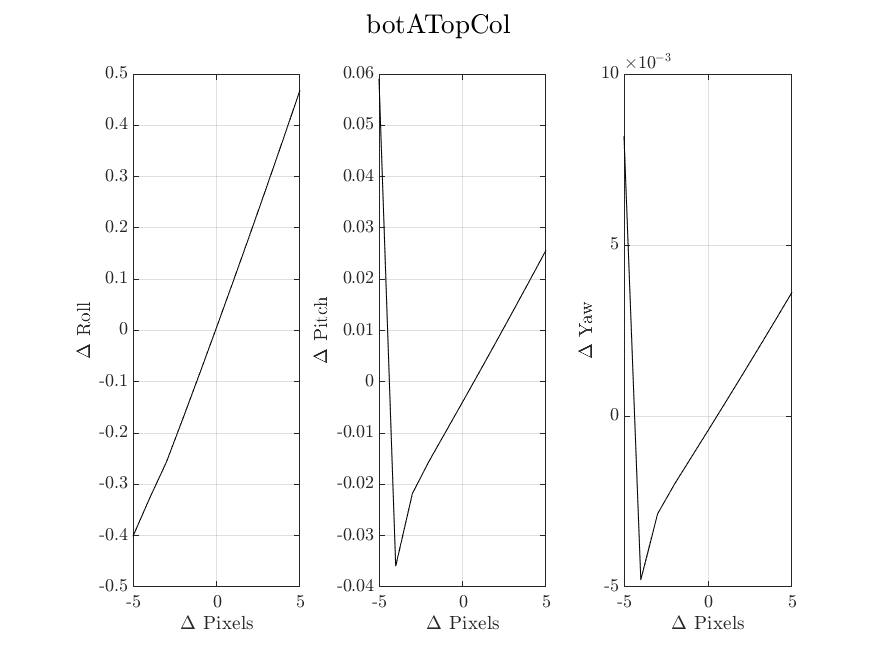
\includegraphics[width=0.9\columnwidth]{botATopCol.png}
	\caption{Bottom A Camera Top Dot, Column\label{fig:botATopCol}}
\end{figure}

\begin{figure}[H]
	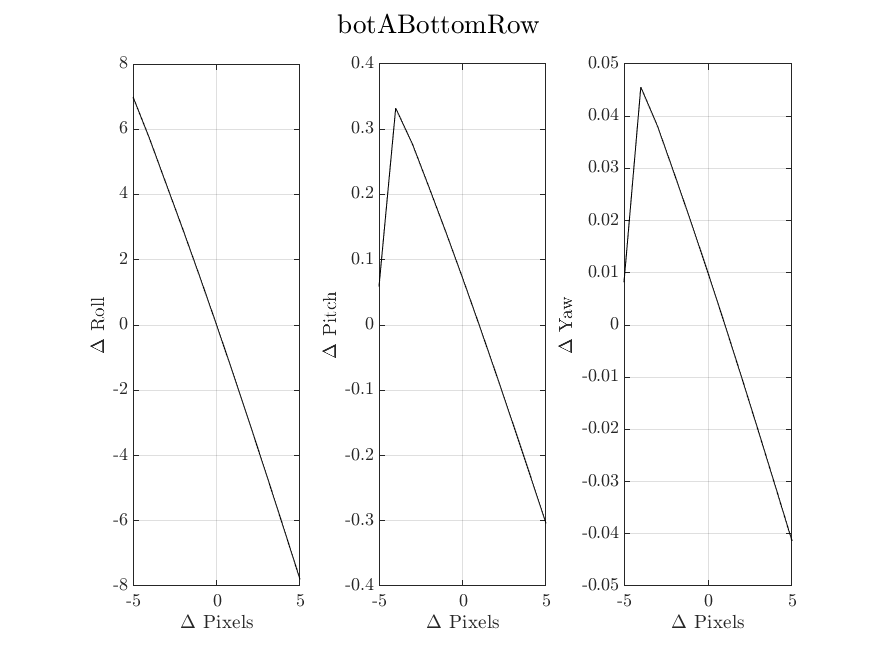
\includegraphics[width=0.9\columnwidth]{botABottomRow.png}
	\caption{Bottom A Camera Bottom Dot, Row\label{fig:botABottomRow}}
\end{figure}

\begin{figure}[H]
	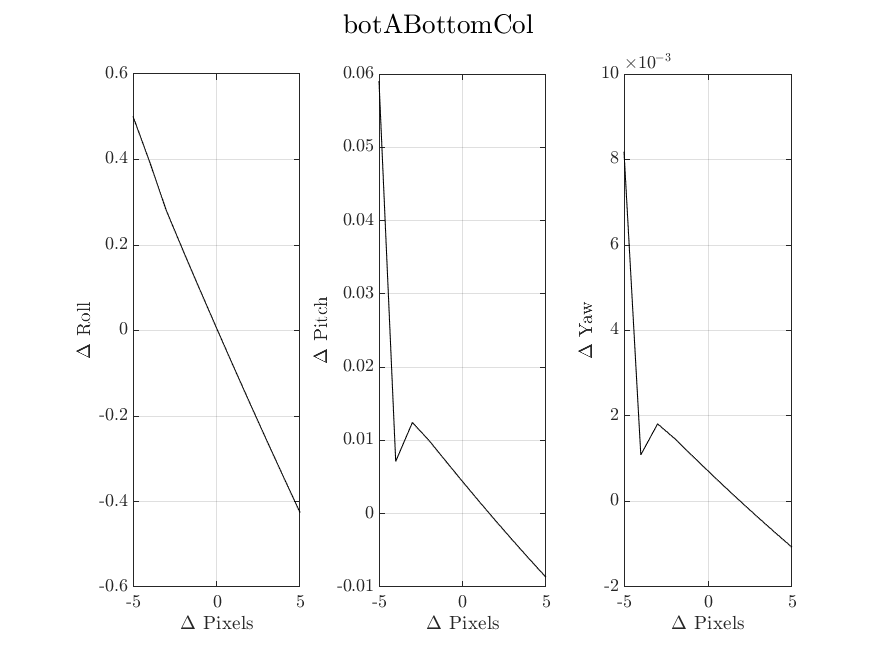
\includegraphics[width=0.9\columnwidth]{botABottomCol.png}
	\caption{Bottom A Camera Bottom Dot, Column\label{fig:botABottomCol}}
\end{figure}

% Bottom B Camera Pixels

\begin{figure}[H]
	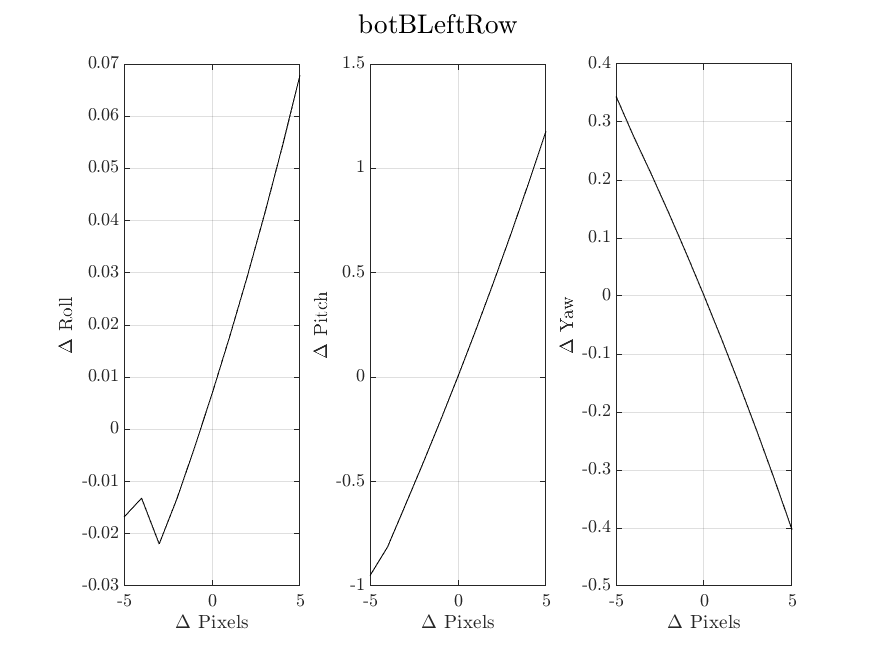
\includegraphics[width=0.9\columnwidth]{botBLeftRow.png}
	\caption{Bottom B Camera Left Dot, Row\label{fig:botBLeftRow}}
\end{figure}

\begin{figure}[H]
	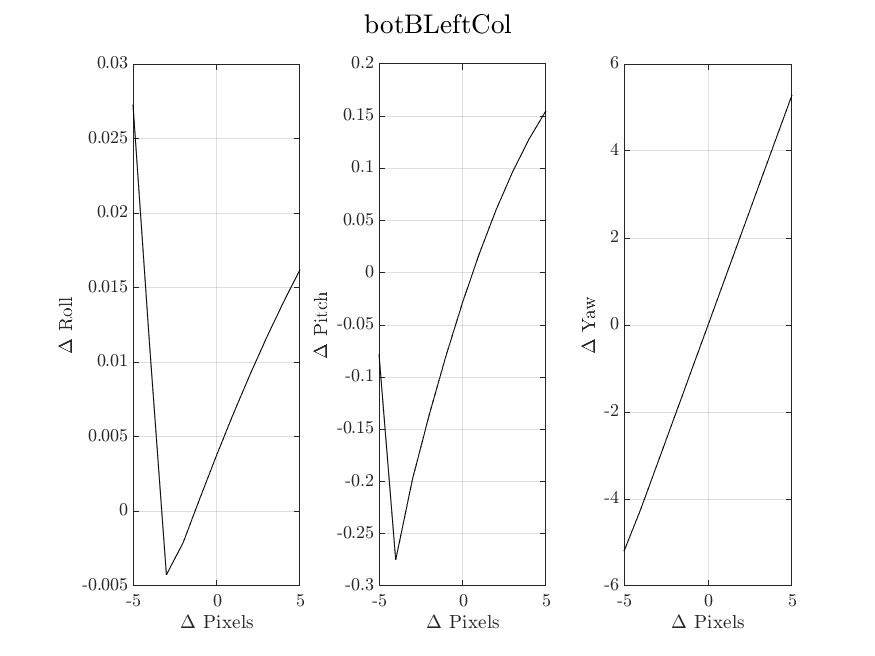
\includegraphics[width=0.9\columnwidth]{botBLeftCol.png}
	\caption{Bottom B Camera Left Dot, Column\label{fig:botBLeftCol}}
\end{figure}

\begin{figure}[H]
	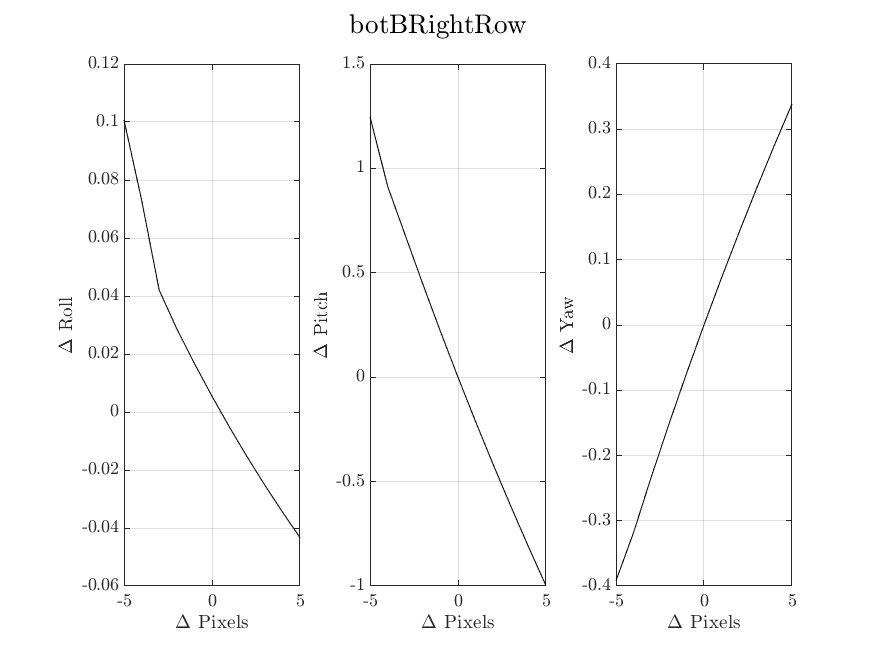
\includegraphics[width=0.9\columnwidth]{botBRightRow.png}
	\caption{Bottom B Camera Right Dot, Row\label{fig:botBRightRow}}
\end{figure}

\begin{figure}[H]
	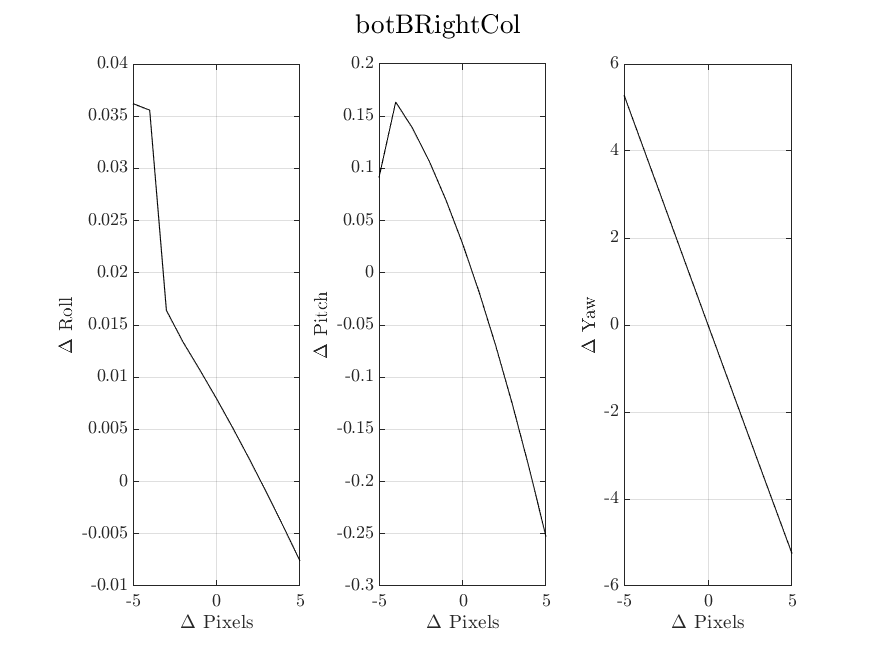
\includegraphics[width=0.9\columnwidth]{botBRightCol.png}
	\caption{Bottom B Camera Right Dot, Column\label{fig:botBRightCol}}
\end{figure}

% Slant Camera Pixels

\begin{figure}[H]
	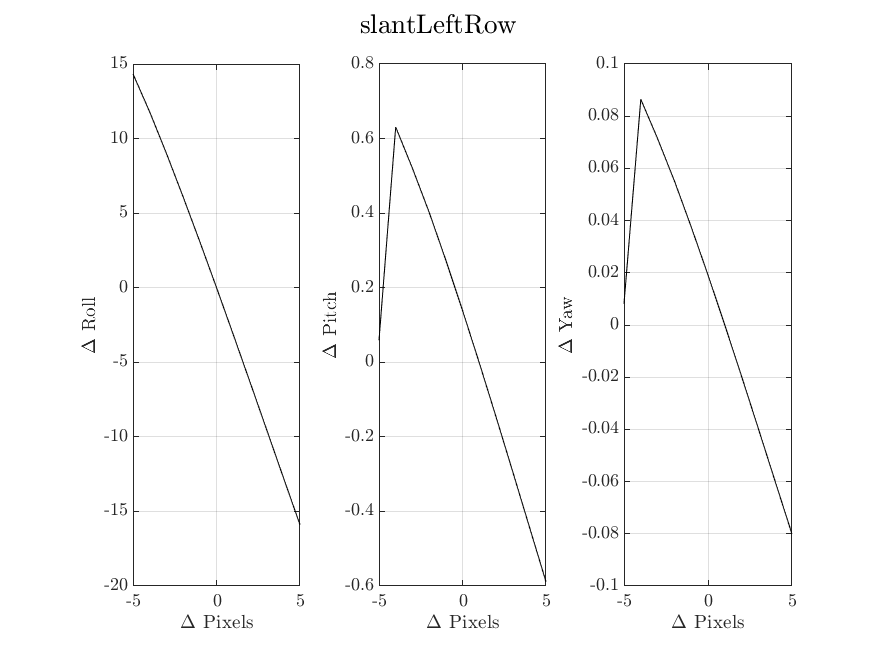
\includegraphics[width=0.9\columnwidth]{slantLeftRow.png}
	\caption{Slant Camera Left Dot, Row\label{fig:slantLeftRow}}
\end{figure}

\begin{figure}[H]
	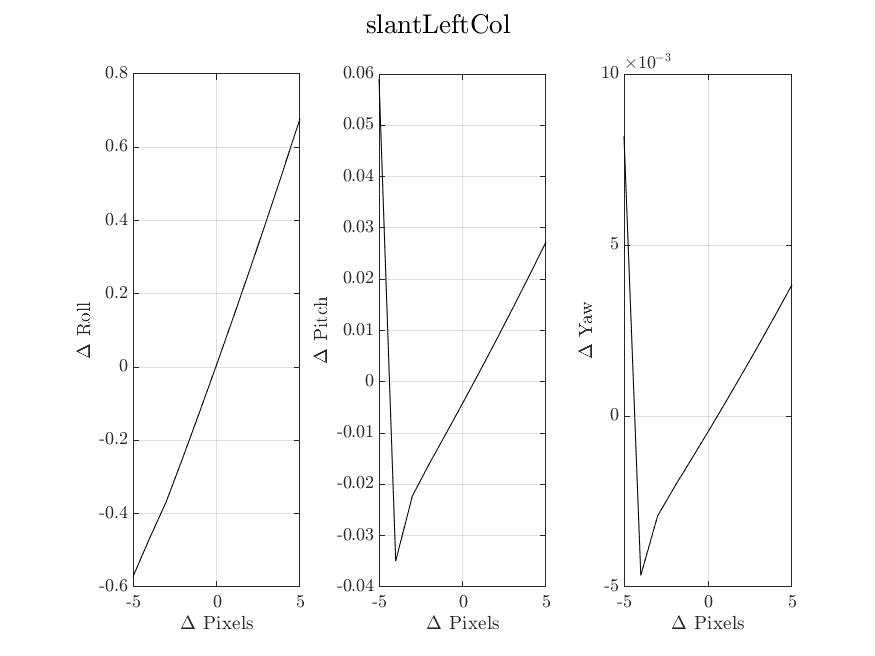
\includegraphics[width=0.9\columnwidth]{slantLeftCol.png}
	\caption{Slant Camera Left Dot, Column\label{fig:slantLeftCol}}
\end{figure}

\begin{figure}[H]
	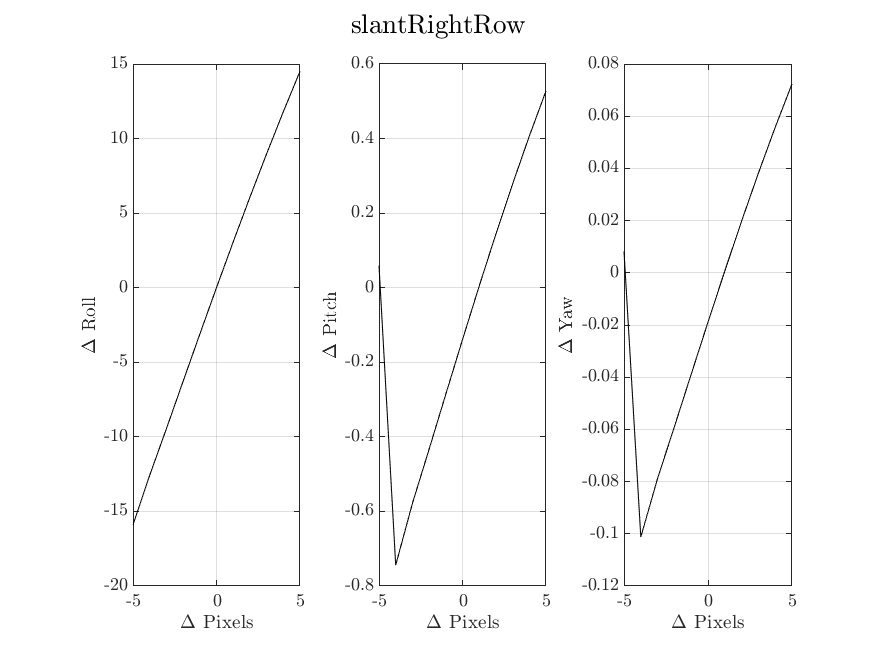
\includegraphics[width=0.9\columnwidth]{slantRightRow.png}
	\caption{Slant Camera Right Dot, Row\label{fig:slantRightRow}}
\end{figure}

\begin{figure}[H]
	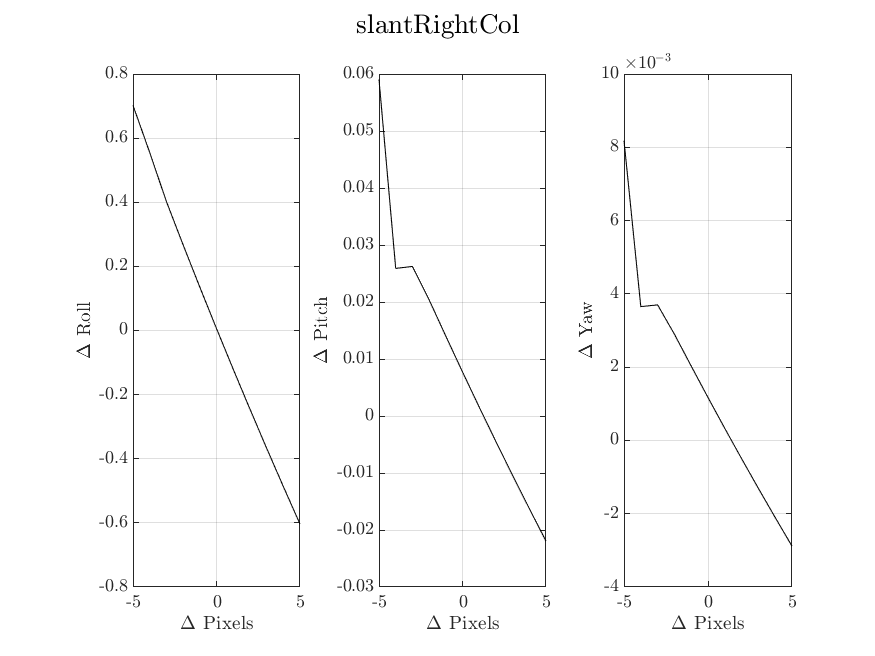
\includegraphics[width=0.9\columnwidth]{slantRightCol.png}
	\caption{Slant Camera Right Dot, Column\label{fig:slantRightCol}}
\end{figure}

\section{Discussion}

What conclusions can we draw, specifically: what was as expected, what was not as expected?

\end{multicols}

\end{document} 
%%%%%%%%%%%%%%%%%%%%%%%%%%%%%%%

This section just contains examples of how to do things
Since it's beyond the document end it shouldn't appear in the final pdf.

Code to create a horizontal line across the page
\noindent\rule{\columnwidth}{0.4pt}

Code to import a table from a .tex file:
\input{../Code/tables/p2GAx0} 

Code to import an m-file
\lstinputlisting{../Code/WM/loadWing.m}

Code to create a figure:
\begin{figure}[H]
	\includegraphics[width=0.48\columnwidth]{../Code/Output/TaperedChordWing_ClDist.png}
	\includegraphics[width=0.48\columnwidth]{../Code/Output/TaperedChordWing_SpanLoad.png}
	\caption{Figure showing $C_l(y)$ obtained from both the lifting line theory code and from the Weissinger method code. \label{fig:TaperedChordWing}}
\end{figure}


Code to manually create a table:
\begin{table}[thpb]
	\centering
	\begin{tabular}{|l|l l|}\hline
		Method: & LLT & WM  \\\hline
		$C_L$   & 1.3382 & 1.2742  \\
		$C_{Di}$  & 0.058034 & 0.051826  \\\hline
	\end{tabular}
	\caption{Distributions $C_l$ and $cC_l/c_{avg}C_L$ as obtained from both the lifting line theory (LLT) code for the tapered wing. \label{tab:TaperedChordWing}}
\end{table}
